\documentclass[10pt]{article}
\usepackage{natbib}
\usepackage{times}
\usepackage[T1]{fontenc}
\usepackage[utf8]{inputenc}
\usepackage[pdftex]{graphicx}
\usepackage{caption}
\captionsetup[figure]{justification=raggedright,labelfont=bf}
\usepackage{fullpage} % 1" margins
\usepackage{setspace}
\setstretch{1.5}
\usepackage{tabu}
%\usepackage{sectsty}
%\sectionfont{\nohang\centering\normalsize\sc}   % capitalize initial letters
%\subsectionfont{\nohang\centering\normalsize\rm\em}

\renewcommand{\thetable}{S\arabic{table}}

% eat the colon so figures are labeled but have blank captions
% \makeatletter
% \renewcommand\fnum@figure[1]{\figurename~\thefigure\ignorespaces}
% \makeatother

%% Article
\begin{document}
\raggedright
\parindent 0.5in


\begin{table}%[tbhp]
  \centering
  \small
  \caption{Global and regional sampling of clades.}
  \begin{tabu} to \textwidth {X[-3,l,b]|X[-1,r,b]X[-1,r,b]X[-1,r,b]|X[-1,r,b]X[-1,r,b]X[-1,r,b]|X[-1,r,b]X[-1,r,b]X[-1,r,b]|X[1,r,b]X[1,r,b]X[1,r,b]}
   \hline
    & \multicolumn{3}{c|}{global} & \multicolumn3{c|}{Hengduan Mountains} & \multicolumn3{c|}{Himalayas-QTP} & \multicolumn3{c}{temperate/boreal East Asia}\\
   clade                                                  & total & sampled & \% & total & sampled & \% & total & sampled & \% & total & sampled & \%  \\
   \hline
   \textit{Acer}                                          & 129   & 118     & 91 & 45    & 29      & 64 & 24    & 15      & 63 & 80    & 72      & 90  \\
   \textit{Allium}                                        & 800   & 378     & 47 & 34    & 29      & 85 & 55    & 37      & 67 & 89    & 100     & 89  \\
   Clematidinae+ Anemoninae                               & 495   & 177     & 36 & 76    & 32      & 42 & 45    & 26      & 58 & 152   & 72      & 47  \\
   Delphineae                                             & 756   & 312     & 41 & 225   & 74      & 33 & 83    & 44      & 53 & 90    & 51      & 57  \\
   \textit{Cyananthus}                                    & 66    & 47      & 71 & 41    & 28      & 68 & 26    & 24      & 92 & 14    & 10      & 71  \\
   \textit{Isodon}                                        & 100   & 63      & 63 & 55    & 40      & 73 & 20    & 9       & 45 & 36    & 24      & 67  \\
   \textit{Ligularia- Cremanthodium- Parasenecio} complex & 380   & 75      & 20 & 152   & 60      & 39 & 62    & 12      & 19 & 148   & 27      & 18  \\
   \textit{Meconopsis}                                    & 54    & 47      & 87 & 25    & 22      & 88 & 36    & 34      & 94 & 2     & 2       & 100 \\
   Microsoroideae                                         & 248   & 147     & 59 & 45    & 42      & 93 & 38    & 35      & 92 & 80    & 66      & 83  \\
   Pinaceae                                               & 234   & 226     & 97 & 34    & 32      & 94 & 26    & 24      & 92 & 63    & 63      & 100 \\
   Polygoneae                                             & 663   & 257     & 39 & 92    & 61      & 66 & 85    & 75      & 88 & 160   & 127     & 79  \\
   Primulaceae                                            & 900   & 354     & 39 & 205   & 114     & 56 & 150   & 68      & 45 & 80    & 55      & 69  \\
   \textit{Rhodiola}                                      & 70    & 57      & 81 & 32    & 28      & 88 & 37    & 30      & 81 & 34    & 20      & 59  \\
   \textit{Rhododendron}                                  & 1000  & 351     & 35 & 237   & 120     & 51 & 124   & 42      & 34 & 300   & 105     & 35  \\
   \textit{Rosa}                                          & 175   & 102     & 58 & 49    & 27      & 55 & 29    & 20      & 69 & 64    & 35      & 55  \\
   \textit{Saussurea}                                     & 416   & 147     & 35 & 108   & 73      & 68 & 130   & 63      & 48 & 157   & 56      & 36  \\
   Saxifragaceae+ Grossulariaceae                         & 760   & 313     & 41 & 209   & 54      & 26 & 155   & 45      & 29 & 170   & 102     & 60  \\
   \textit{Thalictrum}                                    & 150   & 104     & 69 & 38    & 34      & 89 & 40    & 25      & 63 & 48    & 32      & 67  \\
   \hline
    
  \end{tabu}
\end{table}

%%% Local Variables: 
%%% mode: latex
%%% TeX-master: "SI"
%%% End: 


\clearpage
\newpage

\section*{Materials and Methods}

\subsection*{Molecular dating}

We followed three general guidelines in doing molecular
divergence-time estimation.

\begin{enumerate}

\item We use the earliest confirmed fossil record of a group to
  constrain its minimum stem age. This is because most fossil species
  are published based on fragmentary material that lack enough
  characters to be placed within the crown group.

\item We applied uniform priors to all calibrations, despite the
  effect of inferred node age confidence intervals being larger than
  for other commonly-used distributions, e.g.\ lognormal, exponential,
  etc.% We believe current
  % knowledge on fossils only allow us to make an assumption that one
  % clade could originate at any time between the minimum and maximum
  % bounds.

\item We use 125 Myr, the age of the earliest eudicot fossil
  \citep{Hughes1994}, to constrain the maximum age of angiosperm
  clades in the absence of other empirical constraints. As our
  sampling is generally focused on genera and families, this is a
  conservative constraint.

\end{enumerate}

\subsubsection*{Clade 1: \textit{Allium} (Amaryllidaceae)}

There are no reliable fossils for \textit{Allium} or
Amaryllidaceae. However, the containing order Asparagales was dated
with fossil calibrations in a study by \citet{Chen2013}, from which we
extracted two secondary calibrations of Amaryllidaceae.

Root (crown of Amaryllidaceae): The age constraint was set to
42.0--61.7 Myr based the 95\% HPD of the crown age of Amaryllidaceae
from Chen et al. \citep{Chen, Kim et al. 2013}.

Crown of Allioideae: The age constrain was set to 27.8 – 44.5 Myr based the 95% HPD of the crown age of Allioideae from Chen et al. \citep{Chen, Kim et al. 2013}.

Clades 2 and 3: \textit{Ligularia-Cremanthodium-Parasenecio} complex and
\textit{Saussurea} (Asteraceae)

As no reliable fossils for Ligularia-Cremanthodium-Parasenecio complex and Saussurea are available, we estimate their divergence times in two steps. 1) We dated the backbone tree of Asteraceae using reliable fossils. The backbone tree includes 499 genera of Asteraceae with one genus represented by one taxon. Four genera of Calyceraceae were selected as outgroups. 2) We used ages inferred from the first step as secondary calibrations to estimate divergence times of Ligularia-Cremanthodium-Parasenecio complex and Saussurea. 
(1) Step 1: Dating the backbone tree of Asteraceae
Crown of Asteraceae: In a recent study, Barreda et al. \citep{Barreda, Palazzesi et al. 2015} implied a Cretaceous pollen, Tubulifloridites lilliei type A to constrain of the split age of Barnadesia and Dasyphyllum after detailed comparison with extinct and extant Asteraceae. However, the systematic position of T. lilliei type A is still debated \citep{Barreda, Palazzesi et al. 2015, Panero 2015}. Therefore, we use this fossil in a conservative way to constrain the minimum age of the crown of Asteraceae. 
Stem of Asteraceae except Barnadesieae and Famatinanthus: The minimum stem age of this clade was constrained using a well-studied fossil, Raiguenrayum cura \citep{Barreda, Palazzesi et al. 2010, Barreda, Palazzesi et al. 2012}.  It is an exceptionally well preserved capitulescence from the 47.5 Myr old Huitrera Formation in Argentina. Taking together with associated pollen Mutisiapollis, this fossil shared a mosaic of morphological characters of modern groups, such as Stifftieae, Mutisioideae sensu lato and Carduoideae. Therefore, we used it to constrain the minimum stem age of the major Asteraceae.
Stem of Mutisieae: The minimum age of the stem Mutisieae was constrained by the earliest unequivocal fossil pollen for this tribe, Mutisiapollis patersonii, from the early Oligocene of Australia \citep{Macphail and Hill 1994}. M. patersonii is similar to some extant species in Chaetanthera and Mutisia, however, it is unclear whether it can be placed any extant genera. It is safe to constrain the minimum age of the Mutisieae. 
Stem of Nassauvieae: The earliest fossil pollen of this clade, Huanilipollis cabrerii, is found from the early Miocene sediments in South America \citep{Barreda, Palazzesi et al. 2008, Barreda, Palazzesi et al. 2010}. It is similar to pollen of recent Holocheilus, Jungia, and Proustia by being subprolate, tricolporate, microechinate and with a complex exine structure \citep{Barreda, Palazzesi et al. 2008}. To be more conservative, we use it to constrain the minimum age of the stem Nassauvieae.
Stem of Cichorieae except Scorzonerinae: The earliest confirmed fossil pollen of Cichorieae, Cichorium intybus-type pollen was found from the Molasse of the paratethys which is at least 22 Myr old \citep{Hochuli 1978}. The Cichorium intybus-type pollen has three poral lacunae, six abporal lacunae (three at each side of the equator), and six paraporal lacunae (three on each side of the equatorial ridge) \citep{Blackmore 1984} which is widely distributed in all subtribes except Scorzonerinae \citep{Tremetsberger, Gemeinholzer et al. 2013}.
Stem of Sonchus and Launaea: Late Miocene Sonchus oleraceus-type pollen resembles to extant Aetheorhiza, Hyoseris, Launaea, and Sonchus \citep{Blackmore, Van Campo et al. 1986}. As we only sampled Launaea and Sonchus, we use it to constrain the minimum age of stem Sonchus and Launaea.
(2) Step 2: Dating of Ligularia-Cremanthodium-Parasenecio complex and Saussurea based on secondary calibrations from Step 1
Ligularia-Cremanthodium-Parasenecio complex: 
Root: The crown of Ligularia-Cremanthodium-Parasenecio complex is constrained to be 9.5-29.8 Myr.  
Crown of Ligularia: 2.32-16.85 Myr.
Crown of Petasites and Tussilago: 1.09-15.18 Myr. 
Saussurea:
Root (Crown of Saussurea): 2.27-13.98 Myr. 

Clade 4: Cyananthus (Campanulaceae)
As no reliable fossils for Cyananthus and related genera are available, we expanded our sampling to the whole Campanulaceae to date the phylogeny. 
Root (Crown of the Campanulaceae): The crown of the Campanulaceae was constrained by secondary calibration inferred from Magallón et al. \citep{Magallón, Gómez‐Acevedo et al. 2015}. The age range of the root was set to 62 -90 Myr. 
Split between Campanula pyramidalis and C. carpatica: Fossils of C. palaeopyramidalis was used to constrain the stem age of C. pyramidalis and C. carpatica \citep{Lancucka-Srodoniowa 1979}. This fossil taxon was re-evaluated and believed to resemble to C. pyramidalis \citep{Cellinese, Smith et al. 2009}.

Clade 5: Rhodiola (Crassulaceae) 
As no reliable fossils are available for Rhodiola and Crassulaceae, we expanded our sampling to the Saxifragales. One hundred and seventy-one species from the Saxifragales were selected as outgroups. We applied the same fossil calibrations as Saxigragaceae and Grossulariaceae (detailed information see fossil calibrations for Saxifragaceae and Grossulariaceae).
Clade 6: Rhododendron (Ericaceae)
To incorporate more fossil calibrations, we selected several species from Empetrum, Enkianthus, Erica and Kalmia as outgroups.  We mainly use fossil calibrations for Ericaceae selected by Schwery et al. \citep{Schwery, Onstein et al. 2015}. However, to be more conservative, we constrained the stem age rather than the crown age of Rhododendron using the earliest fossil of this genus. This because the earliest fossil cannot be assigned to any subgenus based on morphological characters. We applied the earliest fossil record of Ericaceae (89.8 Myr) to be the maximum age of other calibrations in the Ericaceae.
Root: The minimum age of the root was constrained by the earliest fossil record (89.8 Myr) of Ericaceae, Paleoenkianthus sayrevillensis \citep{Nixon and Crepet 1993}. 
Stem of Rhododendron: The minimum age of the stem of Rhododendron was constrained by the earliest fossil record of this genus, R. newburyanum from the Paleocene of South England \citep{Collinson and Crane 1978}. The age range was set to 56 - 89.8 Myr.
Stem of Erica: The minimum age of the stem of Erica was constrained by the earliest fossil record of this genus, E. palaeoarborea from the late Miocene of Europe \citep{Van der Burgh 1987}. The age range was set to 5.33 - 89.8 Myr. 
Stem of Empetrum: The minimum age of the stem of Empetrum was constrained by the earliest fossil record of this genus, E. sp. from the middle Miocene of Denmark \citep{Friis 1979}. The age range was set to 11.62 -89.8 Myr. 
Stem of Kalmia: The minimum age of the stem of Kalmia was constrained by the earliest fossil record of this genus, K. saxonica from the early Miocene of Germany \citep{Van der Burgh 1987}. The age range was set to 15.97 – 89.8 Myr.
Clade 7: Isodon (Lamiaceae)
The divergence time of Isodon has been well estimated using fossil calibrations by Yu et al. \citep{Yu, Maki et al. 2014}. We used the stem and crown ages of Isodon to calibrate our phylogeny. The stem age of Isodon was set to 17.03 – 39.84 Myr and the crown age was set to 14.66 – 26.44 Myr \citep{Yu, Maki et al. 2014} using uniform priors.
Clade 8: Meconopsis (Papaveraceae)
There is no reliable fossils are available for Meconopsis and Papaveraceae. Xiao \citep{Xiao 2013} estimated the divergence time of Meconopsis based on fossil calibrations from the other Ranunculales. We used her estimated crown age 12 – 34 Myr as secondary calibrations. 
Clade 9: Pinaceae
Root (Crown of the Pinaceae): We applied the earliest fossil cone assigned to Pinaceae, Eathiestrobus to constrain the minimum age of the root of Pinaceae \citep{Rothwell, Mapes et al. 2012}. The maximum age of the root was set to 200 Ma as no putative fossils of Pinaceae before Jurassic so far. We placed three fossil calibrations in Pinaceae selected by Leslie et al. \citep{Leslie, Beaulieu et al. 2012}. We also followed their settings of the lower and upper bounds \citep{Leslie, Beaulieu et al. 2012}, but use uniform priors. 
Stem of Larix: The earliest reliable Larix fossil record, L. altoborealis from middle Eocene of Canada was used to constrain the stem age of Larix \citep{LePage and Basinger 1991}. The age range was set to 41-60 Myr \citep{Leslie, Beaulieu et al. 2012}. 
Stem of Picea: Picea burtonii, the earliest reliable fossil of Picea from the Early Cretaceous Apple Bay locality, Vancouver Island, British Columbia \citep{Klymiuk and Stockey 2012} was used to constrain the stem of Picea.  The age range was set to 133-153 Myr \citep{Leslie, Beaulieu et al. 2012}. 
Stem of Tsuga: Tsuga swedaea from the middle Eocene Buchanan Lake formation, Axel Heiberg island \citep{Lepage 2003} was used to constrain the stem age of Tsuga. The age range was set to 41-100 Myr \citep{Leslie, Beaulieu et al. 2012}.
Clade 10: Polygoneae (Polygonaceae)
Stem of Polygonaceae (root): Polygonocarpum johnsonii Manchester and O’Leary from the Maastrichtian of southwestern North Dakota, USA was used to constrain the minimum age of the stem of Polygonaceae \citep{Manchester and O’Leary 2010}. The fossil fruit possesses fusiform-reticulate venation over the wings and deeply inset intramarginal veins which are known only in Polygonaceae \citep{Manchester and O’Leary 2010}. This fossil calibration was also used to constrain the stem age of Polygonaceae in previous study \citep{Magallón, Gómez‐Acevedo et al. 2015}. The age range was set to 65.5 – 125 Myr.
Stem of Polygonum: The minimum age of stem Polygonum was constrained by the earliest fruit fossil record of Polygonum from the early Oligocene of western Siberia \citep{Dorofeev 1963}. The age range was set to 28.1 – 125 Myr.
Stem of Persicaria: Several Persicaria type fossil pollen records have been reported from Paleocene of Europe \citep{Krutzsch 1970, Gruas-Cavagnetto 1978} and were accepted by Muller \citep{Muller 1981}. The age range was set to 55.8 – 125 Myr.
Stem of Rumex: Reliable Rumex seed and fruit fossils (R. miolusaticus) have been reported from the middle Miocene of Germany \citep{Mai 2001}. Here, we use it to constrain the minimum age of the stem of Rumex. The age range was set to 16 – 125 Myr.
Crown of Muehlenbeckia: We use the 12.7 Myr old Muehlenbeckia fossil from New Zealand \citep{Pole 1993} to calibrate the minimum age of the crown age of Muehlenbeckia. It was assembled to the extant species M. australis \citep{Pole 1993} and this classification was evaluated by expert of Polygonaceae \citep{Schuster, Setaro et al. 2013}. The age range was set to 12.7 – 125 Myr.
Clade 11: Microsoroideae (Polypodiaceae)
We expanded our sampling to the Polypodiaceae to incorporate more fossil calibrations. One hundred and seventy-nine species from Polypodiaceae were selected as outgroups. 
Root (crown of Polypodiaceae): The earliest uncontroversial fossil for the Polypodiaceae from Eocene of Siberia, Protodrynaria takhtajanii \citep{Vikulin and Bobrov 1987}, was used to constrain the minimum age of the crown of Polypodiaceae. The maximum age of Polypodaceae was based on a secondary calibration, the uppermost bound for the Polygrammoids \citep{Schuettpelz and Pryer 2009}. The root age was set to 33.9 -77 Myr.
Crown of Drynaria: The minimum crown age of Drynaria was constrained using the fossil of extant species, D. propinqua which was discovered from the late Miocene flora of SW China \citep{Wen, Xie et al. 2013}. The upper bound was set to be 66 Myr, as the genus is unlikely to origin before the Cenozoic. The crown age of Drynaria was set to 5.3 – 66 Myr.
Stem of Polypodium: The minimum stem age of Polypodium was constrained using the earliest fossil record of this genus from the early Oligocene of Czech Republic \citep{Kvacek 2001}. The stem age of Polypodium was set to 25.6 – 66 Myr.
Stem of Pleopeltis: The oldest reliable fossil of Pleopeltis from the Miocene of Dominican Republic (15.8 – 20.3 Myr) \citep{Schneider, Schmidt et al. 2015} was used to constrain the minimum age of the stem of Pleopeltis. The stem age of Pleopeltis was set to 15.8 – 66 Myr.

Clade 12: Primuloideae (Primulaceae s.s.)
We expanded our sampling to the whole Primulaceae (s. l.). Five fossils were used as calibrations in dating the Primulaceae phylogeny. 
Root (Crown of Primulaceae s. l.): The minimum age of the root was constrained by the earliest fossil record of the Primulaceae (s.l.) assigned to Ardisia which was collected from the early Eocene London Clay Formation (~48.6 Myr) \citep{Collinson 1984}. Fossils of Myrsinoideae have also been reported from the early Eocene United States \citep{Irving and Stuessy 1971}. Maximum ages of the crown age of Primulaceae (s.l.) were constrained by the earliest fossil flowers of the Primuloids which were collected from the Late Cretaceous (Campanian-Maastrichtian) Mira locality of Portugal \citep{Friis, Crane et al. 2011}. The age range of the root was set to 48.6 – 72 Myr.
Stem of Primuloideae (Primulaceae s.s.): The earliest fossils of the Primuloideae which were collected from the early Oligocene Siberia was used to constrain the minimum age for the stem of the Primuloideae \citep{Nikitin 2006}. The stem age range of Primuloideae was set to 28 – 72 Myr.
Stem of Primula: The earliest unequivocal fossil of Primula, P. riosiae from the early-mid Miocene boundary was applied to constrain the minimum age for the stem of Primula \citep{de Vos, Hughes et al. 2014}. The stem age range of Primula was set to 15.96 – 72 Myr.
Stem of Androsace: The earliest fossil seed of Androsace was found from the Miocene western Siberia \citep{Dorofeev 1963}. We use this fossil to constrain the minimum age of Androsace. The stem age range of Androsace was set to 5.3 – 72 Myr.
Clade 13-15: Clematidinae-Anemoninae, Delphineae and Thalictroideae (Ranunculaceae)
The fossil record of Ranunculaceae has been well reviewed by Friis et al. \citep{Friis, Crane et al. 2011} and Pigg and DeVore \citep{Pigg and DeVore 2005}. The Cretaceous record of the Ranunculaceae is sparse. For Delphinea, we expanded our sampling to the whole Ranunculaceae. One hundred and thirty-eight species from other genera of Ranunculaceae were selected as outgroups. 
Root (crown of Ranunculaceae): Pollen of Cretacaeisporites scabratus from the Cretaceous (probably Late Cenomanian) of Gabon is polyporate, showing strong affinity with pollen of some extant Ranunculaceae like Anemone, Coptis, and Hepatica in aperture configuration and tectum ornamentation, and also in pollen wall ultrastructure \citep{Ward and Doyle 1994}. Therefore, we set the minimum age of the root based on this fossil record. The age of the root was set to 93.9 – 125 Myr.
Stem of Actaea: The minimum stem age of Actaea was constrained based on fossil fruits from the late Paleocene of North Dakota, Paleoactaea nagelii \citep{Pigg and DeVore 2005}. The stem age of Actaea was set to 56.8 – 125 Myr.
Stem of Clematis: The minimum stem age of the stem of Clematis was constrained based on the fossil fruits from the Oligocene Germany \citep{Weyland 1938}. The stem age of Clematis was set to 23 – 125 Myr.
We applied all fossil calibrations used for the Delphinae in dating Clematidinae-Anemoninae and Thalictroideae. Besides above fossil calibrations, we added two more calibrations. We used Eocaltha zoophilia from the Campanian of Mexico which show similarity to seeds of extant Caltha to constrain the stem age of Caltha \citep{Rodrı́guez-de la Rosa, Cevallos-Ferriz et al. 1998}. The stem age of Caltha was set to 70.6 – 125 Myr. We applied the Oligocene Ranunculus fossil fruits to constrain the stem age of this genus \citep{Mai 1985}. The stem age of Ranunculus was set to 23 – 125 Myr.
Clade 16: Rosa (Rosaceae)
Rosales has very good fossil record among all the angiosperms \citep{Xing, Gandolfo et al. 2016}. To incorporate more fossil calibrations, we selected 203 taxa from other genera of Rosaceae and four species of Rhamnaceae as outgroup. 
Root (split between Rosaceae and Rhamnaceae): We use the old fossil flower of Rhamnaceae from the late Campanian of Mexico, Coahuilathus belindae \citep{Calvillo-Canadell and Cevallos-Ferriz 2007} to constrain the minimum divergence age between Rosaceae and Rhamnaceae.
Crown of subfamily Spiraeoideae (excl. Lyonothamnus, supertribe: Kerriodae and Tribe: Neilieae): The earliest fossil from this subfamily, Paleorosa from the middle Eocene of British Colombia \citep{Basinger 1976} was used to constrain the minimum age of this clade as it shares feature of both the traditional subfamilies Maloideae and Spiraeoideae. The age range was set to 49.4 – 125 Myr.
Crown of the Tribe Amygdleae: Prunus fossil from the middle Eocene Okanogan Highlands \citep{DeVore and Pigg 2007} can be used to calibrate the stem of Prunus. As Prunus is not monophyletic, we use this fossil to constrain the crown of the Tribe Amygdleae. The age range was set to 49.4 – 125 Myr.
Crown of the Tribe Kerriae: The earliest fossil record for this tribe is assigned to the genus Neviusia which was also discovered from the middle Eocene Okanogan Highlands site \citep{DeVore, Moore et al. 2004}. It was used to constrain the minimum crown age of the Tribe Kerriae. The age range was set to 49.4 – 125 Myr.
Stem of Rosa: The earlies fossil record of Rosa is from the late Eocene Florissant Formation \citep{Manchester 2001}. It was used to constrain the minimum age of the stem Rosa. The age range was set to 34 – 125 Myr.

Clade 17: Acer (Sapindaceae)
Root (Split between Acer and Dipteronia):  The split between Acer and Dipteronia was calibrated using the earliest fossil Dipteronia \citep{McClain and Manchester 2001}. The fossil record of Dipteronia was well reviewed by McClain and Manchester \citep{McClain and Manchester 2001} based on diagnostic winged fruits. We use the earliest Dipteronia fossil from the Paleocene North America to constrain the minimum age of the root. The maximum age was set to 125 Ma.
Crown of Acer: The genus Acer has a rich fossil record dates back at least to Paleocene and Eocene \citep{Wolfe and Tanai 1987, Mai 1995}. The first fossil samaras possibly assignable to section Acer are reported from the latest Early Eocene of North America \citep{Wolfe and Tanai 1987}. We use it to constrain the minimum age the genus Acer and the maximum age was set to 125 Ma. 
Clade 18: Saxifragaceae + Grossulariaceae
We selected five species of Itea and one species of Pterostemon from Saxifragales as outgroups. 
Root: We set the minimum age of the root using the Upper Cretaceous fossil (Turonian, ca. 90 Myr), Divisestylus \citep{Hermsen, Gandolfo et al. 2003}. The phylogenetic position of Divisestylus has been demonstrated based on well preserved morphological characters of flowers and fruits that it shows clear affinity to Iteaceae \citep{Hermsen, Gandolfo et al. 2003}. As it represents the oldest fossil for Iteaceae + Saxifragaceae and cannot be assigned to extant Iteaceae, we used it constrain the root of the phylogeny. The age range of the root was set to 90 – 125 Myr.
Stem of Itea: The fossil record of Iteaceae and Grossulariaceae and their phylogenetic positions have been well reviewed by Hermsen \citep{Hermsen 2013}. Following her arguments, we used the earliest fossil pollen assigned to Itea (49 Myr) to constrain the minimum age of the stem of Itea. The stem age range of Itea was set to 49 – 125 Myr.
Stem of Ribes: The earliest uncontroversial fossil leaves assigned to Ribes axelrodii from the Eocene Bull Run floras (approximately 42 Myr) was used to constrain the minimum age of the stem of Ribes \citep{Hermsen 2005}. The stem age range of Ribes was set to 42 – 125 Myr.


2. Biogeographical range scoring
Data matrices for the geographic ranges of species sampled in the studies clades were assembled mainly based on the online eFloras and databases such as Flora of China (http://www.efloras.org/flora_page.aspx?flora_id=2), Flora of North America (floranorthamerica.org), Flora of Pakistan (http://www.efloras.org/flora_page.aspx?flora_id=5), EURO+MEDI PlantBase (http://www.emplantbase.org/), USDA (plants.usda.gov), annotated checklist of the flowering plants of Nepal (http://www.efloras.org/flora_page.aspx?flora_id=110), and Global Biodiversity Information Facility (GBIF: http://www.gbif.org/) with introduced collections excluded. We obtained a county level distribution for most of Himalayan-Hengduan region species by cross checking with Biodiversity of the Hengduan Mountains database (http://hengduan.huh.harvard.edu), dataset of distributions ranges for species included in Vascular Plants of the Hengduan Mountains compiled by Zhang et al. \citep{Zhang, Boufford et al. 2009}, and Wu \citep{Wu 2008}.
3. Ancestral regions reconstruction

\bibliography{SI-refs}
\bibliographystyle{ecol_let}

% \begin{figure}
% \begin{center}
% 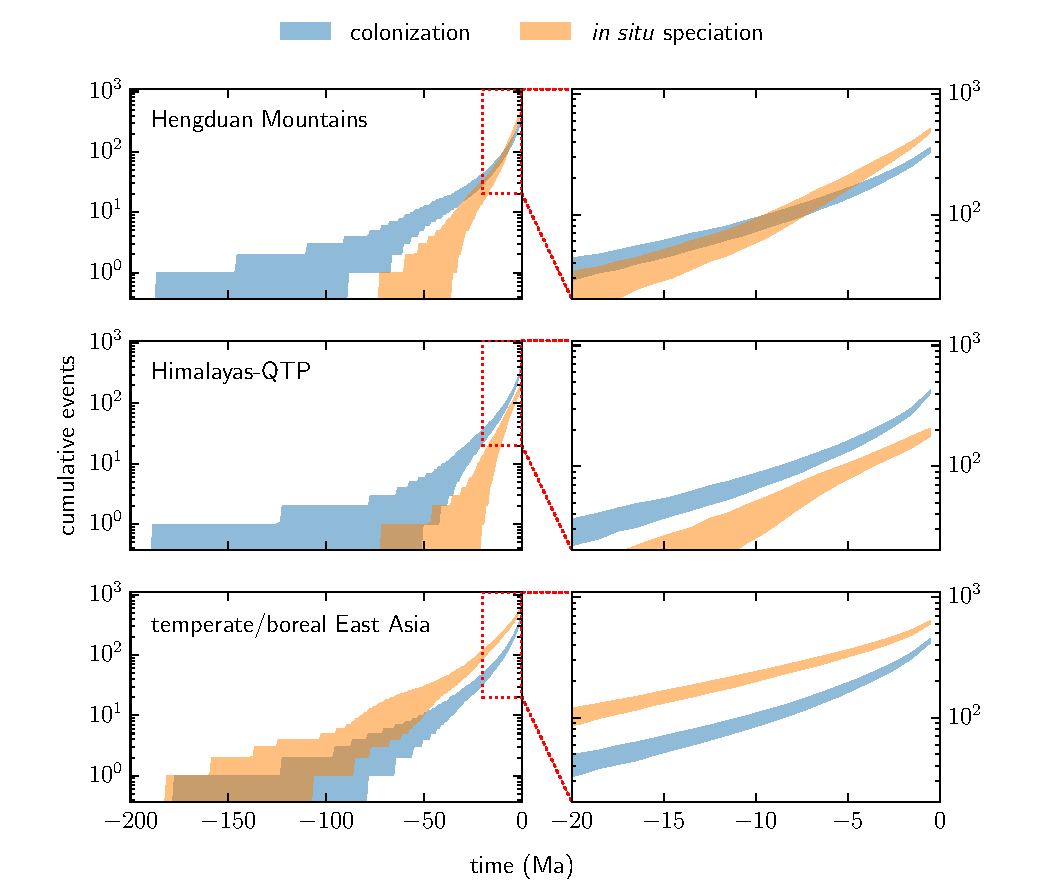
\includegraphics[width=.99\textwidth]{figures/figure_cumulative_events/figure_cumulative_events.pdf}
% \end{center}
% \caption{Assembly of regional floras by colonization and \textit{in situ} speciation events in 18 plant clades, inferred from ancestral-range reconstructions on time-calibrated molecular phylogenies. Shaded regions indicate the 5--95\% quantile intervals for the cumulative number of events through time from 500 pseudoreplicated joint biogeographic histories designed to account for phylogenetic uncertainty (see text). Panels on the right focus on the last 20 Ma, in which differences in regional assembly are most apparent. In the Hengduan Mountains region, cumulative \textit{in situ} speciation overtakes colonization about 8 Ma, whereas for the Himalayas-QTP, colonization remains the dominant process. \textit{In situ} speciation thus appears to have played a disproportionately large role in assembling the Hengduan Mountains flora since the late Miocene compared to the Himalayas-QTP, consistent with the theory of uplift-driven diversification in the Hengduan Mountains region.}
% \label{fig:cumevents}
% \end{figure}

\end{document}

%%% Local Variables:
%%% mode: latex
%%% TeX-master: t
%%% End:
